% !TeX root = ../thuthesis-example.tex

\chapter{驾驶舱简介}

\section{飞行员驾驶舱}

\begin{figure}[htb]
  \center
  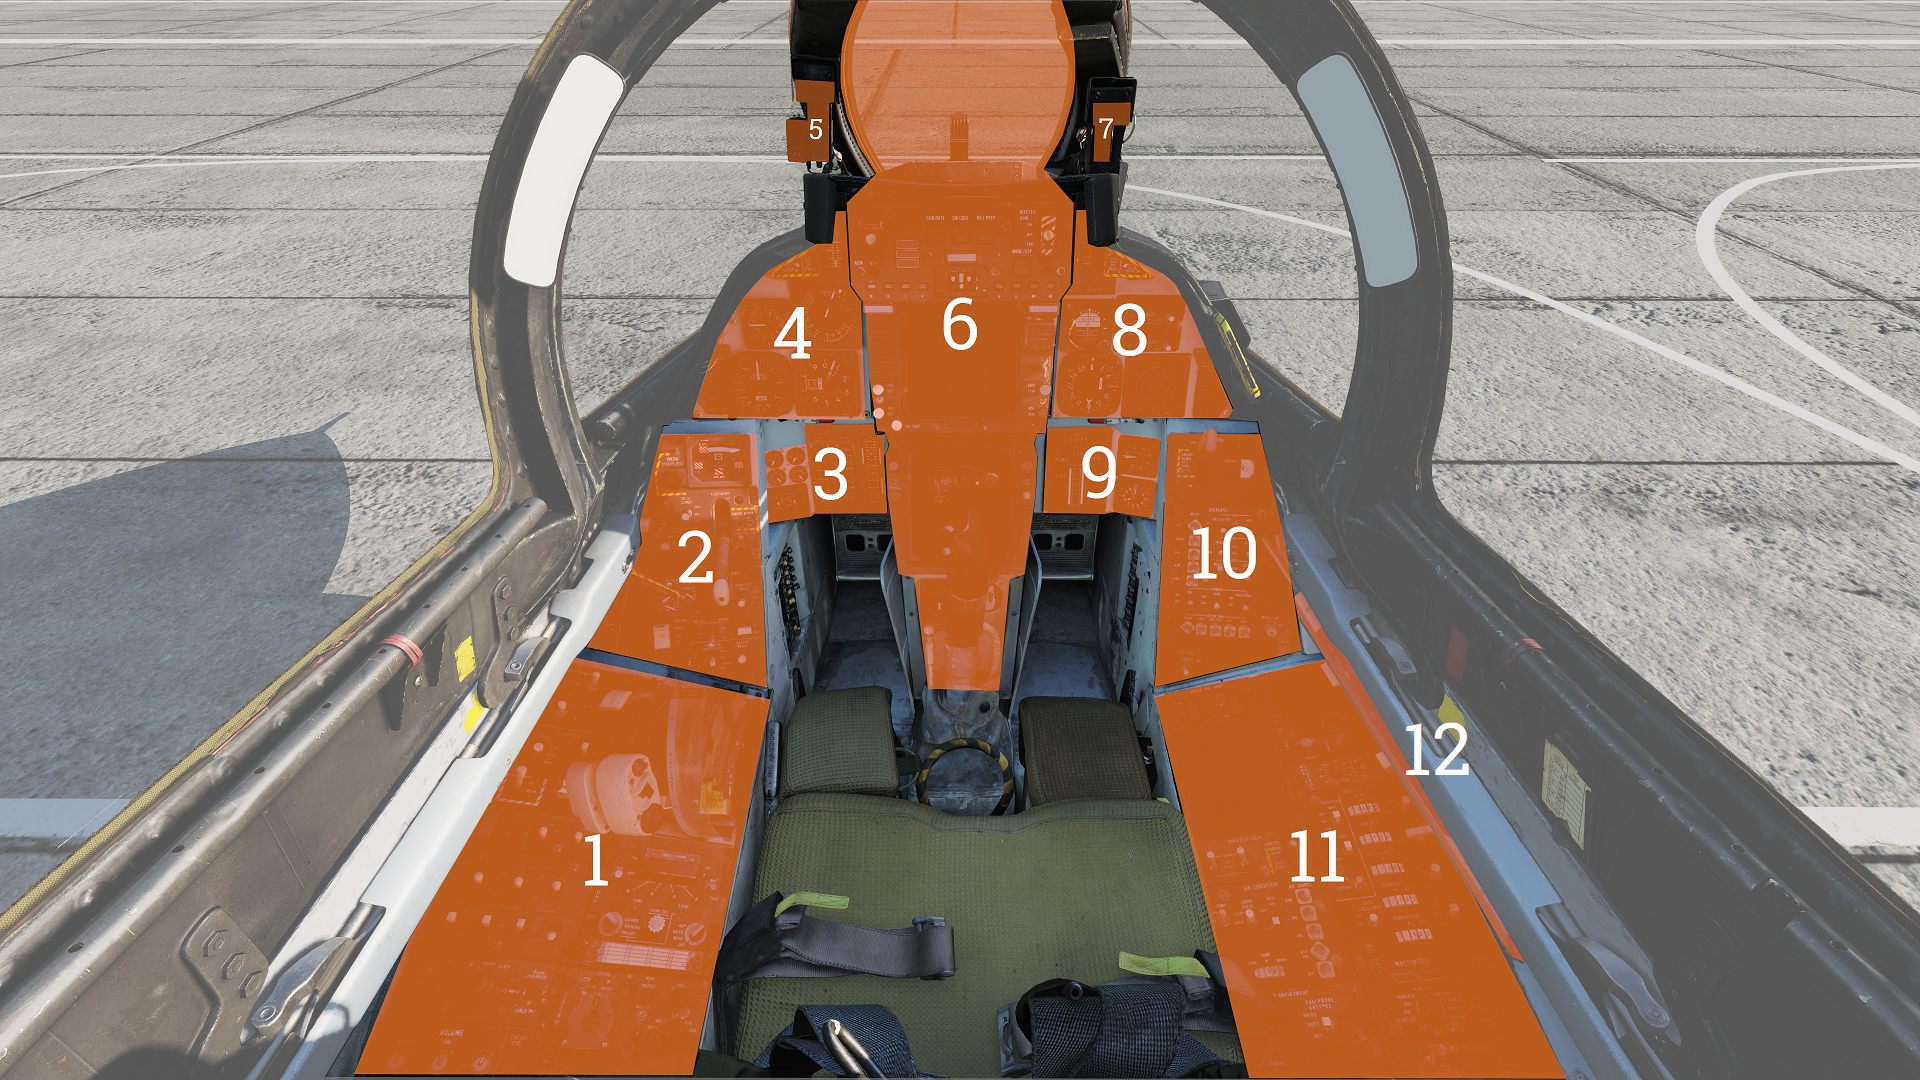
\includegraphics[width=0.6\textwidth]{pilotcockpit.png}
\end{figure}

\subsection{左侧控制台}

\subsubsection{抗荷服充气检测按钮}
\begin{figure}[htb]
  \center
  \includegraphics[width=0.6\textwidth]{g-valve.png}
\end{figure}
按下按钮来测试抗荷服充气。

\subsubsection{供氧-通风控制面板}

\begin{figure}[htb]
  \center
  \includegraphics[width=0.6\textwidth]{oxygen-vent.png}
\end{figure}
控制抗荷服或坐垫中的通风气流以及通向飞行员面罩的氧气。

\begin{enumerate}
  \item VENT AIRFLOW 拨轮:通风气流调节拨盘,用于控制抗荷服气流进出,未连接抗荷服时则控制坐垫气流。
  \item OXYGEN 开关:供氧开关,开关有 ON / OFF 两个档位。用于控制流向面罩的氧气。
\end{enumerate}

\subsubsection{音量/TACAN指令面板}

\begin{figure}[htb]
  \center
  \includegraphics[width=0.6\textwidth]{volume.png}
\end{figure}
用于调整飞行员头戴中的音量和指定控制 TACAN 的乘员。

\begin{enumerate}
  \item ALR-67 旋钮:用于控制飞行员头戴中 ALR-67 的音量。
  \item SW 旋钮:“响尾蛇”音量旋钮,用于调节飞行员头戴中“响尾蛇”导弹的音调音量。
  \item V/UHF 2 旋钮:控制飞行员头戴中 AN/ARC-182 无线电台的音频音量。
  \item TACAN CMD 按钮开关:带有指示灯的按钮开关,用于指定控制 TACAN 设备的乘员(飞行员 / RIO)。指示灯显示当前的设定。
\end{enumerate}

\subsubsection{TACAN控制面板}

\begin{figure}[htb]
  \center
  \includegraphics[width=0.6\textwidth]{tacan.png}
\end{figure}
如果飞行员有 TACAN 设备控制权,则可以通过该控制面板操作 TACAN。

\begin{enumerate}
  \item 双层旋转开关:使用外侧拨盘选择 TACAN 波道的前两位数字,使用内侧拨盘选择最后一位数字。
  \item GO 和 NO-GO 灯:通过/未通过指示灯,指示 TACAN 是否通过自检。
  \item BIT 按钮:自检按钮,按下按钮开始 TACAN 自检。
  \item MODE 开关:波段模式选择开关,用于切换 TACAN 工作波段,可以选择 X 或 Y 波段。INVERSE 模式无功能。
  \item VOL 旋钮:音量旋钮,用于调节飞行员 TACAN 音频音量。
  \item 模式选择旋钮:用户选择TACAN工作模式。
  \begin{itemize}
    \item OFF:关闭 TACAN。
    \item REC:仅接收信号。
    \item T/R:传输并接收信号,该模式下TACAN可以进行测距。
    \item A/A:空对空TACAN模式。
    \item BCN:信标TACAN模式(无功能)。
  \end{itemize}
\end{enumerate}

\subsubsection{机内通话系统控制面板}

\begin{figure}[htb]
  \center
  \includegraphics[width=0.6\textwidth]{ics.png}
\end{figure}
用于控制机内通话系统(ICS)。
\begin{enumerate}
  \item VOL旋钮:音量旋钮,用于调节飞行员接收 RIO 对讲音频的音量。
  \item 放大器选择旋钮:用于选择处理飞行员头戴音频的放大器。
  \begin{itemize}
    \item B/U:备用放大器。
    \item NORM:正常放大器。
    \item EMER:应急放大器。这个档位会使用 RIO 的放大器和他的音量设定。启用应急放大器时,飞行员将无法监听只有常规放大器中飞行员才能听见的 “响尾蛇” 导弹音调和发动机失速 / 超温警告音。
  \end{itemize}
  \item ICS控制开关:用于选择 ICS 的功能。
  \begin{itemize}
    \item RADIO OVERRIDE:无线电台超控,让 ICS 音频替换无线电音频。
    \item HOT MIC:RIO 无需按下 PTT(Push-To-Talk,按键通话)开关即可进行对讲。地勤人员也可以通过外部对讲机与乘员通话。
    \item COLD MIC:RIO 需按下 PTT 开关才能对讲。
  \end{itemize}
\end{enumerate}

\subsubsection{AFCS控制面板}

\begin{figure}[htb]
  \center
  \includegraphics[width=0.6\textwidth]{afcs.png}
\end{figure}
用于控制自动飞控系统(AFCS)和自动驾驶。

\begin{enumerate}
  \item PITCH 开关:启用俯仰通道增稳。
  \item ROLL 开关:启用滚转通道增稳。
  \item YAW 开关:启用偏航通道增稳。
  \item VEC/PCD/ACL 开关:用于切换自动驾驶远程控制模式。
  \begin{itemize}
    \item VEC/PCD:引导航向/精确航线方向模式。数据链路控制飞机滚转和俯仰轴。这个模式通过飞行员驾驶杆上的 NWS(前轮转向)按钮激活。
    \item OFF:功能关闭。
    \item ACL:自动助降模式,这个模式通过飞行员驾驶杆上的 NWS 按钮激活。
  \end{itemize}
  \item ALT开关:高度保持开关,开关有 ALT / OFF 两个档位,用于启用自动驾驶高度保持。这个功能通过飞行员驾驶杆上的 NWS 按钮激活。
  \item HDG开关:航向保持开关,用于选择航向保持模式。
  \begin{itemize}
    \item HDG:启动航向保持模式。
    \item OFF:关闭航向保持模式。
    \item GT:启用地面轨迹模式,通过飞行员驾驶杆上的 NWS 按钮激活。
  \end{itemize}
  \item ENGAGE 开关:自动驾驶控制开关,有 ENGAGE / OFF 两个档位,分别启用和关闭自动驾驶。
\end{enumerate}

\subsubsection{UHF 1(AN/ARC-159)无线电台}

\begin{figure}[htb]
  \center
  \includegraphics[width=0.6\textwidth]{arc-159.png}
\end{figure}
1号 UHF 电台及其控制组件。

\begin{enumerate}
  \item VOL 旋钮:音量旋钮,用于调节飞行员头戴中的 UHF 1 音频音量。
  \item SQL 开关:静噪控制开关,有 ON / OFF 两个档位,分别用于开启或关闭静噪。
  \item 频率选择开关:频率选择拨动开关,用于调定频率。
  \item FREQ./(CHAN) 显示窗:频率 /(波道)显示窗,用于显示当前选中的频率或波道。
  \item READ开关:读取控制开关,按住开关时,频率/(波道)显示窗将显示预设波道的频率。
  \item BRT旋钮:亮度旋钮,用于调节显示屏的亮度。
  \item LOAD按钮:加载按钮,用于加载预设波道的显示频率。
  \item 功能选择旋钮:用于选择无线电功能,该旋钮的四个档位分别是 ADF、BOTH、MAIN 和 OFF。
  \item CHAN SEL旋钮:波道选择旋钮,用于选择预设波道。
  \item 预设波道表:用于记录频率或预设波道的作用。
  \item 模式选择旋钮:这个旋钮用于选择无线电频率模式(GUARD - 救生频率,MANUAL - 手动频率,PRESET - 预设频率)。
  \item TONE按钮:音调按钮,按住按钮会在当前无线电频率上发送一个单音(频率为1,020赫兹)。
\end{enumerate}

注意:AN/ARC-159 中的 ADF 无功能,改为使用 V/UHF 2中的 ADF。

\subsubsection{不对称推力限制器 / 发动机模式选择}

\begin{figure}[htb]
  \center
  \includegraphics[width=0.6\textwidth]{asym.png}
\end{figure}
这个面板用于控制不对称推力限制系统和发动机控制模式。

\begin{enumerate}
  \item ASYM LIMITER 开关:不对称推力限制器开关,带有保护盖,开关 ON / OFF 两个档位分别启用和禁用不对称加力推力限制器。
  \item ENG MODE SELECT 开关:发动机模式选择开关,用于选择左右发动机各自的控制模式。
  \begin{itemize}
    \item PRI:主要控制模式。
    \item SEC:次要控制模式。
  \end{itemize}
\end{enumerate}

\subsubsection{目标指定开关}

\begin{figure}[htb]
  \center
  \includegraphics[width=0.6\textwidth]{target.png}
\end{figure}

用于在 HUD 中指定地面目标,也用于控制飞行员 ACM 雷达模式,但 PLM(飞行员锁定模式)模式除外。开关可以上下拨动,也可以向前拨动至目标指定档位。

空对地模式中,上/下拨动开关来移动指示符,向前拨动开关来指定目标。在其他模式中,上/下拨动开关分别选择 VSL HI(垂直扫描锁定 - 高目标)和VSL LO(垂直扫描锁定 - 低目标)ACM模式,而向前拨动开关选择 PAL 模式。

\subsubsection{进气道斜板 / 油门控制面板}

\begin{figure}[htb]
  \center
  \includegraphics[width=0.6\textwidth]{inlet.png}
\end{figure}

这个面板用于控制多个发动机系统、油门设置以及方向舵配平。

\begin{enumerate}
  \item THROTTLE MODE 开关:油门模式开关,用于选择油门工作模式。
  \begin{itemize}
    \item AUTO:自动模式。
    \item BOOST:助力模式。
    \item MAN:手动模式。
  \end{itemize}
  \item THROTTLE TEMP 开关:油门温控开关,用于选择油门计算机增益。
  \begin{itemize}
    \item HOT:增大标准油门计算机增益。
    \item NORM:使用标准油门计算机增益。
    \item COLD:减小标准油门计算机增益。
  \end{itemize}
  \item INLET RAMPS 开关:进气道斜板开关,用于选择左右发动机各自的进气道斜板工作模式。
  \begin{itemize}
    \item STOW:收起。
    \item ATUO:自动模式。
  \end{itemize}
  \item ENG CRANK 开关:发动机起动开关,用于起动左发动机或右发动机。
  \item BACK UP IGNITION 开关:备用点火开关,用于开启或关闭备用点火。
  \item RUDDER TRIM 开关:方向舵配平开关,用于调整方向舵配平。
\end{enumerate}

\subsubsection{油门握把}

\begin{figure}[htb]
  \center
  \includegraphics[width=0.6\textwidth]{throttle.png}
\end{figure}
油门握把上包括了各种飞行控制和 HOTAS(手不离杆)功能。

\begin{enumerate}
  \item 减速板开关:用于控制减速板展开和收起。
  \begin{itemize}
    \item EXT:释放开关后,回到中间位置。将开关保持在 EXT 档位会逐渐展开减速板。开关回中后,减速板仍会保持在当前位置。
    \item RET:将开关拨至该位置来收起减速板。
  \end{itemize}
  \item 机翼后掠控制开关:这个开关用于控制机翼后掠功能。手动模式下选择的后掠位置只能比 CADC 设置的位置靠后(后掠角度不能小于 CADC 指令后掠角)。
  \begin{itemize}
    \item AUTO:机翼后掠位置由 CADC(中央大气数据计算机) 自动设置。
    \item FWD:手动向前调节机翼后掠位置。
    \item AFT:手动向后调节机翼后掠位置。
    \item BOMB:如果机翼后掠角度小于55°,则将机翼后掠至55°位置。如果 CADC 设置的后掠位置超过55°,则将后掠位置调整至 CADC 设定的角度。
  \end{itemize}
  \item PLM按钮:飞行员锁定模式按钮,用于选择 AWG-9 的 ACM 飞行员锁定模式。也用于在 ACL(自动助降)过程中解除自动驾驶。
  \item CAGE/SEAM按钮:用于控制 AIM-9 导弹 CAGE(导引头解锁)/ SEAM(“响尾蛇”扩展搜索模式) 并启用 AIM-9 导引头锁定。如果启用了 APC(进近推力补偿器),则用于解除 APC。
  \item 机外照明开关:用于控制机外照明。OFF 档位会关闭所有机外照明,并增加进近指示灯亮起度。ON 档位会开启所有机外照明,并减小进近指示灯亮起度。
  \item ICS按键通话开关:通过这个开关,飞行员可以选择在单波道或双波道 V/UHF 下通话,或与 RIO 对讲。
  \begin{itemize}
    \item ICS:与RIO通话。
    \item BOTH:同时在 UHF 1 和 V/UHF 2 频率下通话。
    \item UHF1:在 UHF 1 频率下通话。
    \item UHF2:在 V/UHF 2 频率下通话。
  \end{itemize}
\end{enumerate}

\subsubsection{油门弧座}

\begin{figure}[htb]
  \center
  \includegraphics[width=0.6\textwidth]{throttles-schem.png}
\end{figure}
油门弧座主要组成部分包括:两个发动机油门控制握把、襟翼控制杆和应急机翼后掠手柄,另外也包括油门握把上用于控制 HOTAS 系统的按钮和开关。油门行程中的 OFF(关闭)、IDLE(慢车)和 MIL(军用推力)位置都有限动卡。

将油门从 OFF 位置推到 IDLE 位置会激活点火器并关闭发动机断油装置。油门握把内并未安装弹簧机构,横向推动油门时,握把不会被弹回原位,因此飞行员在弹射起飞时,可以将油门握把置于 MIL(军用推力)档,而不用担心油门位置意外变动,从而导致发动机转速降低。油门弧座左侧,襟翼控制杆的下方装有一个油门阻尼调节杆,用于选择所需的油门移动阻尼。

襟翼控制杆的无级行程的最前段和最后段分别有两个应急档位,一个是应急收上,一个是应急放下。两个应急档位都有限动卡,襟翼控制杆移动至限动卡位置时,需向外推动才能继续移动至应急档位。应急收上档位会强行收起襟翼,超控正常襟翼控制逻辑。应急放下档位无功能。

手动/应急机翼后掠手柄上方有一个保护盖,且手柄通常处于推入并收起的状态。握住手柄顶部,抽出手柄来进行手动机翼后掠控制。请查阅应急模式来获得更多相关信息。

\subsubsection{手动液压泵}

手动液压泵位于油门弧座的内侧,靠近飞行员左腿的位置。液压系统故障时,飞行员通过手动向机轮刹车蓄压器充压来进行制动操作(当起落架手柄处于放下档位时)或伸出受油管。

\subsection{左侧垂直控制台}
\subsubsection{燃油管理面板}

\begin{figure}[htb]
  \center
  \includegraphics[width=0.6\textwidth]{fuel.png}
\end{figure}
这个面板用于控制诸多燃油相关系统、CADC 复位和防滑系统。

\begin{enumerate}
  \item QTY SEL 选择开关:燃油量选择开关,这个滑动弹簧开关用于选择燃油量条状指示器上显示哪个油箱中的燃油量。松开开关后,开关会弹回 FEED 档位。
  \begin{itemize}
    \item FEED:供油油箱,显示供油油箱和机身油箱中的燃油量。
    \item WING:机翼油箱,显示各个机翼油箱中的燃油量。
    \item EXT:副油箱,显示副油箱中的燃油量。
  \end{itemize}
  \item FEED 开关:供油油箱选择开关,用于选择为发动机供油的油箱。保护盖关闭时,开关被锁定在 NORM 档位。
  \item WING/EXT TRANS 开关:机翼/副油箱转移开关,用于控制机翼油箱和副油箱中的燃油转移。
  \begin{itemize}
    \item ORIDE:超控。
    \item AUTO:一般使用的档位。
    \item OFF:停止机翼和副油箱的燃油传输。
  \end{itemize}
  \item 受油管指示灯:当受油管未完全伸出,或未完全收起时,指示灯便会亮起。
  \item DUMP 开关:放油开关,用于开启或停止放油。减速板收起,机轮不负重且加力燃烧关闭时飞机可以进行放油操作。
  \item REFUEL PROBE 开关:受油管开关,用于伸出或收起受油管。
  \begin{itemize}
    \item ALL EXTD:受油管移动至完全伸出位置,允许对所有(ALL)油箱受油。同时也会将机翼/副油箱转移开关(WING/EXT TRANS)复位回 AUTO 档位。
    \item FUS EXTD:受油管移动至完全伸出位置,只允许对机身(FUS)油箱受油。
    \item RET:收起受油管。
  \end{itemize}
  \item ANTI SKID SPOILER BK 开关:防滑和扰流板制动开关,用于选择和控制防滑系统和扰流板制动系统。
  \begin{itemize}
    \item BOTH:机轮负重时,启用防滑系统和扰流板制动系统。
    \item OFF:关闭防滑系统和扰流板制动系统。
    \item SPOILER BK:扰流板制动,机轮负重时,启用扰流板制动功能。
  \end{itemize}
  \item MASTER RESET 按钮:CADC 主复位按钮,用于复位 CADC 故障检测系统及相关故障显示。
  \item 操纵面位置指示器:显示操纵面位置。详见下文。
\end{enumerate}

\subsubsection{操纵面位置指示器}

\begin{figure}[htb]
  \center
  \includegraphics[width=0.6\textwidth]{control.png}
\end{figure}
操纵面位置指示器是用于指示各个飞行操纵面位置的仪表。

\begin{enumerate}
  \item SPOILER 指示器:扰流板位置指示器。
  \begin{itemize}
    \item DN:扰流板收起,与机翼齐平。
    \item 向上箭头:扰流板伸出。
    \item 向下箭头:扰流板放下至机翼表面下方。
  \end{itemize}
  \item RUDDER 指示器:方向舵位置指示器,标注的“L”和“R”分别指示了左方向舵和右方向舵的位置。
  \item HORIZ TAIL 指示器:水平安定面位置指示器,标注的“L”和“R”分别显示了左水平安定面和右水平安定面的位置。
\end{enumerate}

\subsubsection{弹射杆中止面板}

\begin{figure}[htb]
  \center
  \includegraphics[width=0.6\textwidth]{launch-abort.png}
\end{figure}
弹射杆选择开关,将弹簧开关保持在 ABORT 档位时,弹射杆升起,终止弹射。松开开关后,开关弹回 NORM (正常)档位,这也是弹射杆选择开关的标准位置。目前,这个开关在 DCS 中没有实际作用。

\subsubsection{起落架控制面板}

\begin{figure}[htb]
  \center
  \includegraphics[width=0.6\textwidth]{gear.png}
\end{figure}
这个面板用于控制主起落架和应急挂载抛离。

\begin{enumerate}
  \item LDG GEAR 手柄:起落架控制手柄,用于选择起落架的 UP(收上)或 DOWN(放下)位置。紧急情况下(液压失效等),将手柄置于向下位置,并将手柄推入,顺时针旋转手柄顶端然后抽出。这会释放储存的压缩氮气,使起落架紧急放下。
  \item DOWN LOCK ORIDE 杆:起落架放下锁定超控杆,被电磁铁移动至向下位置时指示机轮负重。可以升起至向上位置来超控(起落架手柄锁定在 DOWN 位置)。DCS 中无功能。
  \item HYD ISOL 开关:起落架液压隔离开关,用于将起落架、前轮转向和机轮刹车的液压控制隔离出联合液压系统。起落架手柄处于放下位置时,隔离开关由起落架手柄自动移动至 T.O. / LDG 档位。
  \begin{itemize}
    \item FLT:空中飞行时,隔离上述系统中的液压控制。
    \item T.O. / LDG:起飞/降落,接通上述系统的液压控制,允许它们正常工作。
  \end{itemize}
  \item 起落架位置转移指示灯:起落架实际位置与起落架控制手柄位置不符时,指示灯会亮起。
  \item 机轮-襟翼位置指示器:详见下文。
  \item EMERG STORES 按钮:应急挂载抛离按钮,按下时会亮起,表示激活应急抛离。
  \item NOSE STRUT 开关:前轮支柱开关,这个弹簧开关用于控制前起落架支柱伸缩。
  \begin{itemize}
    \item EXTD:伸展前起落架支柱,升起并锁定弹射杆。
    \item OFF:关闭前起落架支柱运动,松开开关时,开关弹回该位置。
    \item KNEEL:减小前起落架支柱系统中的液压压强,使支柱收缩,从而降低机头的高度,同时解锁弹射杆。
  \end{itemize}
  \item BRAKE-PULL 手柄:制动-抽出手柄,用于控制停放刹车,抽出手柄来启动停放刹车,推入手柄释放机轮刹车。
  \item EJECT CMD 指示器:弹射指令指示器,指示后座驾驶舱的弹射系统的模式。
  \begin{itemize}
    \item PILOT:飞行员弹射时弹射所有机组乘员,RIO 弹射时只弹射自己。
    \item MCO:飞行员或 RIO 弹射时,另一名机组乘员也会被弹射。
  \end{itemize}
\end{enumerate}

\subsubsection{机轮-襟翼位置指示器}

\begin{figure}[htb]
  \center
  \includegraphics[width=0.6\textwidth]{wheels-flaps.png}
\end{figure}

指示襟翼和前缘缝翼、减速板和起落架的位置。前缘缝翼的位置指示标识如下:
\begin{itemize}
  \item \includegraphics[width=1cm, height=1cm]{off.png}:电源切断,或前缘机动缝翼张开。
  \item \includegraphics[width=1cm, height=1cm]{slats-ext.png}:前缘缝翼放下。
  \item \includegraphics[width=1cm, height=1cm]{slats-ret.png}:前缘缝翼收上。
\end{itemize}

在 UP 和 DN 之间移动的指针指示了襟翼的位置。带白色标记的区域指示了机动襟翼的移动范围。起落架位置的指示标识如下:
\begin{itemize}
  \item \includegraphics[width=1cm, height=1cm]{off.png}:电源关闭,或起落架故障(不安全)
  \item \includegraphics[width=1cm, height=1cm]{gear-down.png}:起落架放下。
  \item \includegraphics[width=1cm, height=1cm]{gear-up.png}:起落架收上,起落架舱门关闭。
\end{itemize}

减速板位置的指示标识如下:
\begin{itemize}
  \item \includegraphics[width=1cm, height=1cm]{off.png}:减速板系统电源断开。
  \item \includegraphics[width=1cm, height=1cm]{brake-partial.png}:减速板部分展开,保持位置。
  \item \includegraphics[width=1cm, height=1cm]{brake-out.png}:减速板完全展开。
  \item \includegraphics[width=1cm, height=1cm]{brake-in.png}:减速板收起。
\end{itemize}

\subsection{左膝仪表板}

\subsubsection{液压指示器}

\begin{figure}[htb]
  \center
  \includegraphics[width=0.6\textwidth]{hydraulic.png}
\end{figure}
显示联合液压系统和飞行液压系统的油液压力。SPOIL(扰流板)ON/OFF 警示旗指示外侧扰流板模块加压。选中 EMER FLT(应急飞行液压)HI 或 LOW 时,EMER FLT 标识下方的 HI 和 LOW 对应的 ON/OFF 警示旗分别指示备用飞行液压系统是否启用。

\subsubsection{油压表}

\begin{figure}[htb]
  \center
  \includegraphics[width=0.6\textwidth]{oil.png}
\end{figure}
显示每个发动机的油压。显示范围是 0 到 100 psi,正常范围是 25 至 65 psi,随发动机转速而变化。

\subsubsection{发动机喷口位置表}

\begin{figure}[htb]
  \center
  \includegraphics[width=0.6\textwidth]{exhaust.png}
\end{figure}
显示发动机喷口的位置。显示范围是 0 到 5,指针指向 5 则表示喷口完全张开。

\subsubsection{电子仪表组}

\begin{figure}[htb]
  \center
  \includegraphics[width=0.6\textwidth]{instrument-group.png}
\end{figure}
显示每个发动机的 RPM(高压压缩机转子转速,也就是N2)、EGT(发动机排气温度)和 FF(燃油流量)。

注意:图中展示的是 TF-30 发动机的仪表组,F110 发动机的 EIG 即将实装。
注意:加力推力时 FF 不显示加力消耗的额外燃油。

\subsection{左仪表板}

\subsubsection{雷达高度计}

\begin{figure}[htb]
  \center
  \includegraphics[width=0.6\textwidth]{radaraltimeter.png}
\end{figure}
飞机雷达高度的控制和指示器。

\begin{enumerate}
  \item 雷达高度计控制旋钮:逆时针旋转旋钮至最大位置会关闭雷达高度计。顺时针旋转旋钮来设置警报高度,警报高度随着旋钮顺时针旋转而增加,按下旋钮开始高度表自检。
  \item OFF警示旗:系统关闭、电源关闭或丢失地面锁定时,雷达高度计会显示 OFF 警示旗。
  \item 低高度报警灯:当飞机低于雷达高度计上设置的警报高度时,红灯会亮起。
  \item 自检状态灯:进行高度表自检时,绿灯会亮起。高度表读数应显示100 ± 10 英尺。
\end{enumerate}

低高度限制指示:沿着表盘外沿移动的小三角形游标,它显示了设定的警告高度。
注意:无线电台超控并不会禁用低高度警告的音频。

\subsubsection{气动伺服高度表}

\begin{figure}[htb]
  \center
  \includegraphics[width=0.6\textwidth]{altimeter.png}
\end{figure}
气动伺服高度表的控制和指示器。

\begin{enumerate}
  \item 高度表读数:在机械计数器的三个数位上分别显示万英尺、千英尺和百英尺读数。同时,表盘指针指向的圆形刻度表示百英尺。
  \item 气压调节旋钮:设置以英寸汞柱(in.Hg)为单位的本地气压。只用于气压计本身的读数,所有其他(由 CADC 控制的)数字指示器都使用 29.92 英寸汞柱作为气压数值。
  \item 本地气压:指示调定的本地气压值,这个显示框也被称为“Kollsman Window”。
  \item 模式选择开关:三档位弹簧开关,松开开关时,开关从 RESET 位置弹回正常位置。如果接通电源,且 CADC 可提供高度数据,那么将开关在 RESET 档位保持3秒后,高度计会进入正常(伺服)工作模式。如果将开关拨至 STBY 位置,或电源断开,或缺少 CADC 高度数据,那么3秒后,系统会切换至备用(气压)模式。
\end{enumerate}

STBY 标识旗:如果系统处于备用工作模式,表盘中会显示红色的标有 STBY 字样的标识旗。
注意:	10,000 英尺下高速飞行时,由于气压变化较大,飞机跨声速飞行时,气压计读数误差最多 1,200 英尺,而超声速飞行时,误差可能高达 4,000 英尺 。

\subsubsection{空速马赫表}

\begin{figure}[htb]
  \center
  \includegraphics[width=0.6\textwidth]{mach.png}
\end{figure}
用于指示空速和马赫数。

\begin{enumerate}
  \item 空速表拨盘:用三种刻度显示指示空速,其中两种刻度对应指示空速,另一种刻度则是随着指针拨盘镂空处转动而显示的马赫数。
  \item 指示空速刻度(外圈):指示空速的读数,最高200节。
  \item 指示空速刻度(内圈):指示空速的读数,刻度对应从200节到850节空速。内圈的指示空速刻度被空速表拨盘未镂空的部分盖住,直到需要显示对应的空速时。
  \item 马赫数刻度:马赫数的读数。显示正确的以马赫数为单位的指示空速。
  \item 指示空速游标:可以将游标调定到所需的指示空速上。
  \item 马赫数游标:可以将游标调定到所需的马赫数上。在上图中不可见。
  \item 最大安全马赫数游标:显示 CADC 计算的最大安全马赫数。
  \item 游标设置旋钮:这个旋钮有抽出和按下两个档位,分别用于设置指示空速游标和马赫数游标。
\end{enumerate}

\subsubsection{垂直速率表}

\begin{figure}[htb]
  \center
  \includegraphics[width=0.6\textwidth]{vvi.png}
\end{figure}
显示以前英尺为单位的垂直速率。高度急剧或突然改变时,由于飞机静压口表面的气流快速变化,垂直速率表读数可能产生巨大误差。

\subsubsection{左发断油手柄}

\begin{figure}[htb]
  \center
  \includegraphics[width=0.6\textwidth]{leftengineshutoff.png}
\end{figure}
紧急情况下,抽出手柄来切断左发动机供油。将手柄推入正常位置来重新向发动机注入燃油。但这个手柄不应用于(降落后)关闭发动机。

左发灭火按钮在手柄后方,抽出手柄后方可使用灭火按钮。

\subsubsection{迎角指示器}

\begin{figure}[htb]
  \center
  \includegraphics[width=0.6\textwidth]{aoa.png}
\end{figure}
条形迎角指示器指示了飞机的迎角(AoA),范围是 0 至 30 迎角单位(对应迎角探头在 -10° 至 +40° 范围内转动)。

指示器右侧的标识分别指示各个飞行阶段对应的最佳迎角单位:爬升(5)、巡航(8.5)和失速(29),而 15 单位处的参考横线表示最佳进近迎角单位(15)。

\subsection{风挡左边框}

\subsubsection{进近应交分度器}

\begin{figure}[htb]
  \center
  \includegraphics[width=0.6\textwidth]{aoaindexer.png}
\end{figure}
进近指示灯由三盏灯组成,它显示了当前迎角和最佳进近迎角的相对关系。

绿色灯表示空速过低,琥珀色灯表示正处于最佳进近迎角,而红色表示空速过高。

如果拦阻钩旁路开关处于 CARRIER(着舰)位置,起落架放下,但拦阻钩升起时,进近迎角指示灯会闪烁。

这些灯光会在前起落架支柱的进近灯上重复显示,以便在着舰时,让 LSO(着舰信号官)也能通过观察灯光来判断飞机的 AOA。

\subsubsection{机轮警告/刹车警告/ ACLS 和 AP 注意/ NWS 启用注意/自动油门注意灯}

\begin{figure}[htb]
  \center
  \includegraphics[width=0.6\textwidth]{lefthudcaution.png}
\end{figure}
位于 HUD 左侧的指示灯。

\begin{enumerate}
  \item WHEELS:机轮报警灯。起落架未放下或未锁定,且襟翼放下的角度小于10°,或油门行程小于总行程的85\%时,报警指示灯亮起起。
  \item BRAKES:机轮刹车报警灯。报警指示灯亮起起时,表示防滑系统或刹车故障。设置机轮刹车也会使报警指示灯亮起起。
  \item ACLS/AP:自动助降系统/自动驾驶注意灯。注意指示灯亮起起指示 ACLS 或自动驾驶已断开。
  \item NWS ENGA:前起落架转向激活注意灯。注意指示灯亮起起表示前轮转向已启用。
  \item AUTO THROT:自动油门注意灯。通过油门控制面板上的油门模式开关可以断开自动油门控制,任何其他原因导致的自动油门断开都会使注意指示灯亮起起。
\end{enumerate}


\subsection{中央仪表板}

\subsubsection{平视显示器(HUD)}

\begin{figure}[htb]
  \center
  \includegraphics[width=0.6\textwidth]{hud.png}
\end{figure}
平视显示器用于在驾驶舱前部/风挡玻璃上投影飞行和武器投放数据。使用位于 VDI 右侧的 FILTER 手柄可以选择 HUD 夜间模式。

HUD 的左侧和右侧分别装有失速报警灯(L STALL 和 R STALL 报警灯)。它们分别指示对应一侧发动机的压气机失速。

注意:请查阅 导航 和 武器系统和武器使用总览 来获得更多相关信息。

\subsubsection{驾驶舱电视传感器}

\begin{figure}[htb]
  \center
  \includegraphics[width=0.6\textwidth]{ctvs.png}
\end{figure}
驾驶舱电视传感器(CTVS)录制 HUD 视频,用于记录武器投放信息。

注意:DCS 中未实现此功能。

\subsubsection{空战格斗面板}

\begin{figure}[htb]
  \center
  \includegraphics[width=0.6\textwidth]{acm.png}
\end{figure}
飞行员主要的武器控制面板。

\begin{enumerate}
  \item ACM 开关 / 保护盖:升起 ACM(空战格斗)保护盖会激活 ACM 模式并允许使用 ACM 抛离按钮。
  \item ACM 抛离按钮:ACM 保护盖开关下的抛离按钮用于抛离 RIO 武器控制面板上选择的挂载。按下抛离按钮并不会抛离“响尾蛇”导弹,即使 RIO 选择了“响尾蛇”。
  \item SEAM LOCK 注意灯:当“响尾蛇”导弹处于隶属模式或视轴 SEAM 模式下,且导引头正进行搜索时,SEAM LOCK 灯会亮起。SEAM LOCK 灯会在 SEAM 尝试进行锁定的4.5秒期间内亮起,如果导引头成功锁定目标则继续保持亮起。
  \item COLLISION 注意灯:灯光亮起表示 AWG-9 STT(单目标跟踪)操作时选择了恒量角度拦截转向模式。
  \item HOT TRIG 报警灯:红指示灯亮起起表示满足武器发射逻辑的条件(HOT TRIGGER)。指示灯亮起时,按下扳机会发射武器。
  \item GUN RATE 按钮开关:航炮射速选择开关,用于切换航炮射速模式,开关中的指示灯显示了当前选择的模式,进入 ACM 模式后系统会自动选择 HIGH 模式。
  \begin{itemize}
    \item HIGH:高射速,选择6,000发每分钟的航炮射速。通常用于空对空攻击。
    \item LOW:低射速,选择4,000发每分钟的航炮射速。通常用于空对地攻击。
  \end{itemize}
  \item SW COOL 按钮开关:“响尾蛇”冷却开关,这是一个带有指示灯的按钮开关。按下开关来手动开启或关闭“响尾蛇”导弹冷却。ACM 下将自动切换至 ON(开启)。
  \item MSL PREP 按钮开关:导弹发射准备开关,这是一个带有指示灯的按钮开关。按下开关来命令 WCS(武器控制系统)开始 AIM-54 和 AIM-7 导弹的发射准备过程。ACM 模式下系统将自动切换至 ON。
  \item MSL MODE 按钮开关:导弹模式选择开关,这是一个带有指示灯的按钮开关。用于选择导弹发射模式: NORM(正常)模式或 BRSIT(视轴)模式。在 ACM 模式下,导弹发射模式由 WCS 控制。
  \item MASTER ARM 开关:主军械开关,开启主军械开关将允许武器发射和挂载选择抛离。注意,MASTER ARM(主军械)总线控制与起落架控制手柄互锁,起落架放下时,将禁用除紧急抛离以外的所有发射电路。	主军械开关并不会禁用 ACM 和应急抛离功能。
  \begin{itemize}
    \item OFF:切断武器发射电路的电源。
    \item ON:接通武器发射电路的电源。主军械保护盖升起后才可选择该档位。
    \item TNG(训练):启用飞行训练模式。
  \end{itemize}
  \item 挂点状态标识旗:显示每个挂点的武器状态。
  \begin{itemize}
    \item 黑色:挂点未挂载武器,或武器未就绪。
    \item 白色:挂点和武器准备就绪。
    \item 黑白相间的棋盘图案:该挂点上的武器被选中,且准备发射。在地面时,该图案表示机身导轨挂点升起并锁定,且挂载的武器已激活。
  \end{itemize}
  \item MASTER CAUTION 按钮灯:主注意灯,灯光闪烁表示飞行员注意/提示灯面板上灯光状态发生变化。按下来复位主注意灯并熄灭灯光,直到下一个注意事件被触发。
  \item L FIRE 和 R FIRE 报警灯:发动机火警报警灯。发动机失火时,对应故障发动机一侧的报警指示灯亮起起。
  \item 转弯侧滑指示器:显示飞机围绕垂直轴的转弯率。转弯侧滑仪上半部分是一个电动指针,一个指针距离的偏转等同于4分钟内进行转向一周。转弯侧滑仪下半部分是一个测斜仪,内有一个用于指示侧滑的悬浮在阻尼液中的小球。
\end{enumerate}

\subsubsection{垂直显示指示器(VDI)}

\begin{figure}[htb]
  \center
  \includegraphics[width=0.6\textwidth]{vdi.png}
\end{figure}
为 HUD 补充显示飞行和武器数据。

\begin{enumerate}
  \item HUD 亮度控制旋钮:用于控制 HUD 的亮度。
  \item VDI 亮度控制旋钮:用于控制 VDI 的亮度。
  \item VDI 对比度控制旋钮:用于控制 VDI 的对比度。
  \item FILTER 拉手:抽出手柄以选择 HUD 夜间模式。
  \item HUD TRIM 旋钮:HUD 调节旋钮,使用这个旋钮来调整 HUD 上的俯仰梯度。
  \item VDI TRIM 旋钮:VDI 调节旋钮,使用这个旋钮来调整 VDI 上的俯仰梯度。
  \item VDI 注意灯:VDI 两侧安装的注意灯。详见下文图片和表格。
\end{enumerate}

注意:	点击 VDI 屏幕中央可以加装一个夜间滤镜片。

注意:	请查阅 导航 和 武器系统和武器使用总览 来获得更多相关信息。

\begin{figure}[htb]
  \center
  \includegraphics[width=0.6\textwidth]{vdicaution.png}
\end{figure}
安装在 VDI 面板上的数据链路警告和注意灯。

\begin{enumerate}
  \item ADJ A/C:提示灯,指示有其他飞机接近本机当前的起降航线。
  \item LANDING CHK:提示灯,指示母舰 ACL 通道准备就绪,且机组成员应做好着舰准备。
  \item ACL READY:报警灯,指示 CATCC(母舰空中交通管制中心)已经获取本机信息,且正在向本机传输下滑道信息。
  \item A/P CPLR:报警灯,指示 CATCC 已准备控制飞机。
  \item CMD CONTROL:报警灯,指示飞机正由数据链路控制进行助降。
  \item 10 SECONDS:报警灯,指示 ACL 着舰过程中,数据链路的下滑道信息和指令正根据母舰的持续运动进行调整。在其他模式下则表示距离进近航线钟的下一个检查点还有10秒钟。
  \item TILT:报警灯,指示 ACL 过程中,未能接收数据链路控制的时间超2秒。非 ACL 模式下,报警指示灯亮起起表示过去的10秒内未接收任何数据链路信息。
  \item VOICE:报警灯,指示 CATCC 自动助降未就绪,切换至标准的基于音频通讯的进近流程。
  \item A/P REF:报警灯,指示已选择自动驾驶,但自动驾驶未启用(高度和航向保持除外)。
  \item WAVEOFF:报警灯,指示执行复飞指令。
  \item WING SWEEP:指示指示灯亮起起表示两侧的机翼后掠控制通道中出现故障,或表示应急机翼后掠手柄的随动限位器解除。
  \item REDUCE SPEED:报警灯,指示空速超过225节但襟翼故障无法收上。也用于指示飞机空速超过最大安全马赫数。
  \item ALT LOW:无功能,改用无线电高度计上的灯光。
\end{enumerate}

\subsubsection{水平状态显示器(HSD)}

\begin{figure}[htb]
  \center
  \includegraphics[width=0.6\textwidth]{HSD.png}
\end{figure}
水平状态显示器用于向飞行员显示导航信息。它也用于重复 RIO 的 TID 屏幕中显示的内容。

\begin{enumerate}
  \item BRT 旋钮:亮度旋钮,用于控制 HSD 的亮度。
  \item HDG 旋钮:航向选择旋钮,用于 TACAN 模式下设定参考航向游标。
  \item CRS 旋钮:航线旋钮,用于在 TACAN 和 MAN(手动)模式下设定所需航线。
  \item TEST 按钮:测试按钮,如果触发了过载保护,HSD 显示消失,则可以通过这个按钮来复位 HSD 显示。同时也用于在 HSD 上显示 HSD IR 现场测试。
  \item 自检状态指示灯:显示白色标识旗时,表示 HSD 故障。逆时针旋转旋钮来复位 HSD。
\end{enumerate}

注意:	请查阅 导航 和 战术信息显示器(TID)与相关控制器 中的相关章节来获取更多相关信息。

\subsubsection{座舱压力高度表}

\begin{figure}[htb]
  \center
  \includegraphics[width=0.6\textwidth]{cabinpressure.png}
\end{figure}
以千英尺为单位显示从0至50,000英尺的座舱气压高度。

\subsubsection{应急刹车压力表}

\begin{figure}[htb]
  \center
  \includegraphics[width=0.6\textwidth]{brakepressure.png}
\end{figure}
显示应急刹车蓄压器中的可用于备用刹车和停放刹车系统的油液压力。

PARK - 显示停放刹车可用的刹车压强。绿色区域对应的范围是2,150至3,000 psi(磅力每平方英寸),红色区域对应的范围是1,900至2,150 psi。指针指向绿色时,蓄压器中的液压压强可供刹车进行约三次制动操作。

AUX - 显示备用刹车系统中的刹车压强,飞行员可以通过脚踏上的指尖刹车来启用备用刹车。绿色区域对应的范围是2,150至3,000 psi(约可提供13至14次刹车制动),而红色区域对应的范围则是1,900至2,150 psi(约可提供5次刹车制动)。

\subsubsection{驾驶杆}

\begin{figure}[htb]
  \center
  \includegraphics[width=0.6\textwidth]{stick.png}
\end{figure}
用于控制飞机滚转和俯仰。同时也用于控制下表所述的各种功能:

\begin{enumerate}
  \item 炸弹投放按钮:挂载投放按钮,用于投放空对地挂载(火箭弹例外)或发射挂架挂载的电子对抗措施。
  \item 俯仰和滚转配平开关:这个苦力帽开关用于控制配平,上下位置配平俯仰,左右位置配平滚转。
  \item 武器选择开关:选择开关可上下移动,也可按下。
  \begin{itemize}
    \item SP / PH:选择 AIM-7 或 AIM-54,按下开关来切换选中的导弹类型。
    \item SW:选择 AIM-9,按下开关来切换选中的 AIM-9 挂点。
    \item GUN:选择M-61A1“火神”航炮。
    \item OFF:禁止武器发射。
  \end{itemize}
  \item DLC 和机动襟翼控制拨轮:拨轮用于控制 DLC(直接升力控制)或机动襟翼。启用 DLC 时,向前转动拨轮伸出扰流板,向后转动拨轮收起扰流板。起落架和襟翼收上且 DLC 解除时,向前转动拨轮收起机动襟翼/缝翼,向后转动拨轮放下襟翼。这个功能背后的逻辑是,向后拨动拨轮来增加升力,向前拨动拨轮来减小升力。
  \item DLC 启用/解除和电子对抗措施弹射按钮:襟翼放下,油门不超过 MIL(军用推力)位置,且扰流板系统无故障时,短按按钮来启用 DLC。襟翼收上时,按下按钮会命令 ALE-39 根据 RIO 的设置弹射箔条和红外干扰弹。再次按下按钮,或收起襟翼,或将油门推至超过 MIL 位置,DLC 便会解除。
  \item 自动驾驶接通和前轮转向按钮:机轮负重时,按下按钮来启用或关闭前轮转向系统。机轮不负重时,按下按钮来启用当前选定的自动驾驶模式。
  \item 自动驾驶应急断开手柄:断开所有自动驾驶模式和 DLC,同时将所有自动驾驶模式开关弹回中置位置,并将滚转和俯仰 SAS(增稳系统)开关退回 OFF 位置。机轮负重时,按下紧急断开开关也会将油门模式退回 MAN(手动)模式。
  \item 武器发射扳机:两段式扳机。第一段激活 CTVS(驾驶舱电视传感器)和照相枪。第二段发射选中的前射武器。
\end{enumerate}
注意:DCS 中未实现 CTVS 的功能。

\subsection{风挡右边框}

\subsubsection{ECM(电子对抗)报警灯光}

\begin{figure}[htb]
  \center
  \includegraphics[width=0.6\textwidth]{rwrcaution.png}
\end{figure}
这些报警灯与 ALR-67 相连,用于指示不同类型的雷达威胁。

\begin{itemize}
  \item SAM:地空导弹,灯光稳定亮起表示侦测到地空导弹跟踪雷达锁定,灯光闪烁表示侦测到地空导弹发射。
  \item AAA:防空高炮,灯光稳定亮起表示侦测到防空炮跟踪雷达锁定,灯光闪烁表示侦测到防空炮开火。
  \item AI:机载拦截雷达,灯光稳定亮起表示侦测到机载雷达锁定。
\end{itemize}

\subsubsection{备用罗盘}

\begin{figure}[htb]
  \center
  \includegraphics[width=0.6\textwidth]{compass.png}
\end{figure}
常规备用罗盘。

\subsection{右仪表板}

\subsubsection{机翼后掠指示器}

\begin{figure}[htb]
  \center
  \includegraphics[width=0.6\textwidth]{wingsweep.png}
\end{figure}
用于显示后掠翼系统的详细状态。

最左侧的指针指示了机翼后掠控制程序选定的后掠位置,也就是当前的空速和高度下的最小后掠角度。

中间的条形指示器显示了指令后掠位置。

最右侧指示条指示了实际的机翼后掠位置。

右侧五个垂直排列的显示窗口显示了当前的机翼后掠工作模式。

\subsubsection{右发断油手柄}

\begin{figure}[htb]
  \center
  \includegraphics[width=0.6\textwidth]{rightengineshutoff.png}
\end{figure}
紧急情况下,抽出手柄来切断右发动机供油。将手柄推入正常位置来重新向发动机注入燃油。但这个手柄不应用于正常关闭发动机。

右发灭火按钮在手柄后方,抽出手柄后方可使用灭火按钮。

\subsubsection{备用姿态仪}

\begin{figure}[htb]
  \center
  \includegraphics[width=0.6\textwidth]{standbyattitude.png}
\end{figure}
独立工作的备用姿态仪。

表盘左侧显示的 OFF 标识旗表示备用姿态仪锁定或未通电。

表盘右下方的旋钮用于锁定/解锁姿态仪和调节俯仰梯度显示。旋钮抽出时,姿态仪锁定。旋钮按下时,旋转旋钮可以调节俯仰梯度指示线。

\subsubsection{UHF/VHF 远程显示器}

\begin{figure}[htb]
  \center
  \includegraphics[width=0.6\textwidth]{frontremote.png}
\end{figure}
这个远程显示器用于显示 UHF 1(AN/ARC-159)和 V/UHF 2(AN/ARC-182)中调定的频率或波道。

\begin{enumerate}
  \item UHF 1 远程波道/频率显示器(飞行员):显示 UHF 1 无线电台调定的频率或波道。
  \begin{itemize}
    \item TEST:开始显示器自检,如果通过测试,屏幕中会显示 888.888。
    \item DIM:用于控制显示器亮度。
  \end{itemize}
  \item V/UHF 2 远程波道/频率指示器(飞行员):显示 V/UHF 2 无线电台调定的频率或波道。
  \begin{itemize}
    \item TEST:开始显示器自检,如果通过测试,屏幕中会显示 888.888。
    \item DIM:用于控制显示器亮度。
  \end{itemize}
\end{enumerate}

\subsubsection{方位距离航向指示器(BDHI)}

\begin{figure}[htb]
  \center
  \includegraphics[width=0.6\textwidth]{bdhi.png}
\end{figure}
用于显示方位角和航向信息。

\begin{enumerate}
  \item 二号方位指针:指向调定的 TACAN 台的磁航向。
  \item 罗盘指针:显示当前飞机的磁航向。
  \item 一号方位指针:指向调定的 UHF/ADF 电台的方位。
  \item 距离计数器:显示本机至调定的 TACAN 台的斜距(图中不可见)。
\end{enumerate}

\subsubsection{ALR-67显示器}

\begin{figure}[htb]
  \center
  \includegraphics[width=0.6\textwidth]{alr-67.png}
\end{figure}
用于显示 ALR-67 RWR(雷达告警接收机)组件侦测到的辐射源。

\begin{enumerate}
  \item 系统状态圈
  \begin{itemize}
    \item 左上象限:显示的符号代表威胁目标的显示类型。
    \begin{itemize}
      \item N:正常优先级。
      \item I:AI,优先显示机载拦截雷达威胁。
      \item A:AAA,优先显示防空高炮威胁。
      \item U:优先显示未知辐射源。
      \item F:显示其他雷达威胁的同时也显示友方信号源。
    \end{itemize}
    \item 右上象限:显示 ARL-67 是否处于限制模式。
    \begin{itemize}
      \item 无显示:未选择限制模式。
      \item L:选用限制模式,只显示威胁最高的6个雷达威胁。
    \end{itemize}
    \item 下班部分:显示故障编码,或指示是否启用了威胁目标符号偏置。
    \begin{itemize}
      \item 无显示:无故障且未选择符号偏置。
      \item B:BIT(自检)未通过。
      \item T:过热。
      \item O:选择了偏置显示模式。重叠的威胁目标符号会偏置显示,以增强可读性。选择偏置显示模式时,显示器指示目标方位信息的精度会下降。
    \end{itemize}
  \end{itemize}
  \item 非致命威胁区:用于显示 RWR 认为处于射程外,或未装备武器,从而不直接对本机构成威胁的辐射源。
  \item 致命威胁区:用于显示 RWR 认为处于射程内,且装备武器,但并未攻击本机的辐射源。
  \item 严重威胁区:显示对本机构成直接威胁的辐射源。辐射源有能力攻击本机,且攻击意图明显。
  \item 亮度控制旋钮:用于控制显示器的亮度。
\end{enumerate}

\subsubsection{座舱盖抛离手柄}

\begin{figure}[htb]
  \center
  \includegraphics[width=0.6\textwidth]{canopyjettison.png}
\end{figure}
用于手动抛离座舱盖。

\subsection{右膝仪表板}

\subsubsection{燃油量指示器}

\begin{figure}[htb]
  \center
  \includegraphics[width=0.6\textwidth]{fuelquantity.png}
\end{figure}
用于显示飞机不同油箱中的燃油量。

\begin{enumerate}
  \item BINGO 油量显示:显示当前调定的 BINGO 油量(返航油量)。
  \item TOTAL 总油量显示:燃油总量读数对应了飞机所有油箱中的燃油总量。
  \item L \& R 油量显示:分别用于显示左侧或右侧选定油箱的燃油量。使用燃油管理面板中的 QTY SEL 开关可以选择计数器显示哪一个油箱(供油油箱组、机翼油箱或副油箱)中的燃油量。
  \item FUS \& FEED(机身油箱和供油油箱)指示带:显示对应油箱中的燃油量。左指示带指示左供油油箱组和后机身油箱中的燃油量。右指示带指示右供油油箱组和前机身油箱中的燃油量。
  \item BINGO 设置旋钮:用于选择返航油量(BINGO),旋转旋钮来调定所需油量。
\end{enumerate}

\subsubsection{加速度表}

\begin{figure}[htb]
  \center
  \includegraphics[width=0.6\textwidth]{accelerometer.png}
\end{figure}
显示当前飞机过载值(沿飞机垂直轴的加速度)的仪表。它的显示范围是 -5G 至 +10G。 其中一个指针将显示当前 G 值,而另外两个指针指示飞行过程中受到的最大正 G 和负 G 过载值。 按下仪器左下角的复位按钮可以复位指针位置。

\subsubsection{时钟}

\begin{figure}[htb]
  \center
  \includegraphics[width=0.6\textwidth]{clock.png}
\end{figure}
机械发条时钟。

左下角的旋钮用于上紧时钟发条,顺时针旋转旋钮,然后抽出旋钮来设置时针和分针。

右上角的按钮用于开始、停止和复位时长为1小时的计时器。

\subsection{右侧垂直控制台}

\subsubsection{阻拦钩控制面板}

\begin{figure}[htb]
  \center
  \includegraphics[width=0.6\textwidth]{hook.png}
\end{figure}
用于控制拦阻钩。

\begin{enumerate}
  \item HOOK 手柄:拦阻钩控制手柄,用于选择拦阻钩的位置。
  \begin{itemize}
    \item UP:电动向液压系统增压,升起拦阻钩并上锁。 
    \item DN:电动向液压系统减压,使拦阻钩受缓冲器压力和自身重力放下。
    \item EMERG DOWN:应急放钩,抽出并逆时针旋转手柄会释放拦阻钩锁定机构,使拦阻钩放下。
  \end{itemize}
  \item 拦阻钩过渡指示灯:灯光亮起表示拦阻钩实际位置与拦阻钩手柄对应位置不符。高速飞行中放下拦阻钩时,由于空气向后吹动拦阻钩,使其无法放下,因此指示灯直到拦阻钩完全放下才会熄灭。
  \item 航炮弹药计数器:显示 M-61A1 航炮的剩余弹药数量。从 676 开始倒数,但可按需使用右侧的旋钮调整至所需数值。
\end{enumerate}

\subsubsection{显示控制面板}

\begin{figure}[htb]
  \center
  \includegraphics[width=0.6\textwidth]{displays.png}
\end{figure}
用于控制前座驾驶舱中的显示器。

\begin{enumerate}
  \item STEER CMD 选择开关:转向指令选择开关,用于选择当前的转向指令来源,且所有选择开关互斥(只能选中一个),当前被选中的开关会旋转。
  \begin{itemize}
    \item TACAN:使用 TACAN 作为转向指令源。
    \item DEST:选择 RIO 设置的航路点作为转向指令源。
    \item AWL/PCD:全天候着舰/精确航线方向。按下开关选择使用下滑道引导(ILS/ACLS)进行着舰,或选择PCD作为空对地攻击方向用于转向指令源。
    \item VEC:引导航向,选择数据偏差转向作为转向指令源。
    \item MAN:手动,使用手动选择的航线和航向作为转向指令源。
  \end{itemize}
  \item 用于选择显示模式,且所有选择开关互斥(只能选中一个),当前被选中的开关会旋转。
  \begin{itemize}
    \item T.O.:选择起飞模式。
    \item CRUISE:选择巡航模式。
    \item A/A:选择空对空模式。
    \item A/G:选择空对地模式。
    \item LDG:选择降落模式。
  \end{itemize}
  \item HUD DECLUTTER 开关:HUD 防拥开关,选择 HUD 标识防拥模式。
  \item HUD AWL 开关:选择在 HUD 上显示何种 AWL(全天候降落)信息。
  \begin{itemize}
    \item ILS:选择 ILS 作为 AWL 信息来源。
    \item ACL:选择 ACL 作为 AWL 信息来源。
  \end{itemize}
  \item VDI MODE 开关:VDI 模式选择开关,用于选择 VDI 显示何种数据。
  \begin{itemize}
    \item TV:在 VDI 上显示 TCS 或 LANTIRN 吊舱的视频。
    \item NORM:使用正常 VDI 显示。
  \end{itemize}
  \item VDI AWL 开关:选择 VDI 上显示何种 AWL 信息。
  \begin{itemize}
    \item ILS:选择 ILS 作为 AWL 信息来源。
    \item ACL:选择 ACL 作为 AWL 信息来源。
  \end{itemize}
  \item HSD MODE 开关:HSD 模式选择开关,选择 HSD 上显示何种数据。
  \begin{itemize}
    \item NAV:导航显示,HSD 将根据选定的转向指令源显示转向信息。
    \item TID:重复显示 RIO 的 TID 中的图像。如果 RIO 将 TID 设置显示 TV 图像,则 HSD 无显示。
  \end{itemize}
  \item POWER 开关:电源控制开关,用于控制 VDI、HUD 和 HSD / ECMD 的电源。
  \item PITCH LAD BRT 旋钮:俯仰梯度亮度旋钮,用于控制 HUD 中俯仰梯度线的亮度。
\end{enumerate}
注意:图像资料显示,装有整合 RWR 的 F-14 的 HSD 模式和还有第三种选项——ECM ORDIE(ECM超控),但 Heatblur 的F-14B并没有模拟此选项。

\subsubsection{准星偏移量设置面板}

\begin{figure}[htb]
  \center
  \includegraphics[width=0.6\textwidth]{gunelevation.png}
\end{figure}
用于设置航炮 A/A 和 A/G 模式下准星的抬高/下压量。最小和最大值分别是 -263 和 +87 毫弧度。

\subsection{右侧控制台}

\subsubsection{扰流板故障超控}

\begin{figure}[htb]
  \center
  \includegraphics[width=0.6\textwidth]{spoiler.png}
\end{figure}
用于超控部分故障的扰流板,使其余扰流板在进行 MASTER RESET(大气数据计算机复位)后继续正常工作。

\begin{enumerate}
  \item INBD:内侧扰流板超控开关。
  \begin{itemize}
    \item ORIDE:超控内侧扰流板对称保护,如果一侧扰流板故障,CADC 复位后,允许另一侧正常工作的内侧扰流板继续作动。
    \item NORM:正常模式(保护开关锁定),该模式下,如果一侧的内扰流板故障无法升起,其余扰流板会降下,且注意灯面板中的 SPOILERS 指示灯亮起起。
  \end{itemize}
  \item OUTBD:外侧扰流板超控开关。
  \begin{itemize}
    \item ORIDE:超控外侧扰流板对称保护,如果一侧扰流板故障,CADC 复位后,允许另一侧正常工作的外侧扰流板继续作动。
    \item NORM:正常模式(保护开关锁定),该模式下,如果一侧的外扰流板故障无法升起,其余扰流板会降下,且注意灯面板中的 SPOILERS 指示灯亮起起。
  \end{itemize}
\end{enumerate}

\subsubsection{液氧储量表}

\begin{figure}[htb]
  \center
  \includegraphics[width=0.6\textwidth]{liquidoxygen.png}
\end{figure}
显示了剩余的液氧储备量。每个刻度代表 1 公升。电源故障时,表盘上显示 OFF 标识旗。通过主测试面板的 INST 模式来测试这个仪表,测试时,仪表读数应为 2 公升。

\subsubsection{罗盘控制面板}

\begin{figure}[htb]
  \center
  \includegraphics[width=0.6\textwidth]{compasscontrol.png}
\end{figure}
用于在使用 AHRS(姿态航向基准系统)时选择罗盘工作模式。

\begin{enumerate}
  \item SYNC IND:这个指示器用于显示 AHRS 陀螺仪与磁方位探测器之间是否同步。用于 SLAVED(隶属)模式。
  \item N-S 选择开关:用于选择 DG(航向陀螺仪)和 SLAVED 模式下飞机所处的半球。这个开关对修正地球自转导致的陀螺仪偏移至关重要。
  \item LAT 旋钮:纬度选择旋钮,用于选择从0°到90°的维度,以使 DG 和 SLAVED 模式中的陀螺仪能修正地球自转导致的偏移。
  \item 模式选择开关:用于选择 AHRS 航向信息来源。
  \begin{itemize}
    \item COMP:罗盘,直接使用磁方位探测器,不通过航向陀螺稳定,仅用于紧急情况,且罗盘显示的读数自动使用手动输入的磁差。
    \item SLAVED:正常模式,使用由航向陀螺稳定的磁方位探测器。
    \item DG:航向陀螺仪模式。
  \end{itemize}
  \item HDG 旋钮/按钮:航向选择旋钮,用于 DG 和 SLAVED 模式。在 SLAVED 模式下,它用于同步航向陀螺仪和磁方位探测器,以及设置 BDHI 上的磁航向。按下旋钮,直到同步完成,指示器指针位于零位标记上方。在 DG 模式下,按下并旋转旋钮来调定 BDHI 中的所需航向。按下超过3分钟时,这个旋钮也可以用于快速调平 AHRS 的俯仰和滚转。等待1分钟后,可重新进行调平。
\end{enumerate}

\subsubsection{ARA-63 控制面板}

\begin{figure}[htb]
  \center
  \includegraphics[width=0.6\textwidth]{ara-63.png}
\end{figure}
用于控制 AN/ARA-63 ILS(ICLS)系统。

\begin{enumerate}
  \item CHANNEL 选择开关:波道选择开关,用于从 20 个可用的波道中选择 ICLS 波道。
  \item BIT 按钮:用于测试 AN/ARA-63。如果 VDI 设置就绪,HUD 中会显示助降标识符。
  \item POWER 开关:电源开关,ON/OFF 档位分别用于接通或断开 ARA-63 的电源。提起开关才可将其拨至 OFF 档位。
  \item 状态指示灯:灯光亮起表示 AN/ARA-63 通电。
\end{enumerate}

\subsubsection{注意-提示灯面板}

\begin{figure}[htb]
  \center
  \includegraphics[width=0.6\textwidth]{caution.png}
\end{figure}
飞行员驾驶舱的主要注意灯光面板。

\begin{itemize}
  \item PITCH STAB 1 和 PITCH STAB 2:“俯仰增稳 1” 和 “俯仰增稳 2” 注意灯,指示灯亮起表示俯仰通道不可用。
  \item ROLL STAB 1 和 ROLL STAB 2:“滚转增稳 1” 和 “滚转增稳 2” 注意灯,指示灯亮起表示滚转通道不可用(滚转增稳故障)。
  \item YAW STAB OP:“偏航增稳工作” 注意灯,指示灯亮起表示偏航通道不可用。
  \item YAW STAB OUT:“偏航增稳失效” 注意灯,指示灯亮起表示两个偏航通道不可用(横向增稳故障)。
  \item EMERG JETT:“应急抛离” 注意灯,指示灯亮起表示 EMERG STORES JETT(应急挂载抛离)按钮按下。
  \item LADDER:“登机梯” 注意灯,指示灯亮起表示登机梯未正确折叠收起。
  \item ECS TURBINE:“环境控制系统涡轮” 注意灯,无功能。
  \item INLET ICE:“进气道结冰” 注意灯,注意灯亮起表示结冰信号器探测到结冰。
  \item FLAP:“襟翼” 注意灯,指示灯亮起表示襟翼系统故障,或空速超过225节但襟翼仍未收上。
  \item HZ TAIL AUTH:“水平安定面控制” 注意灯,指示灯亮起表示水平安定面控制作动器故障(或 CADC 故障)。
  \item RUDDER AUTH:“垂尾控制” 注意灯,指示灯亮起表示方向舵控制作动器故障(或 CADC 故障)。
  \item SPOILERS:“扰流板” 注意灯,指示灯亮起表示扰流板系统故障导致多个或全部扰流板锁死。
  \item AUTO PILOT:“自动驾驶” 注意灯,指示灯亮起表示自动驾驶系统故障。
  \item L INLET 和 R INLET:“左进气” 和 “右进气” 注意灯,指示灯亮起表示 AICS(进气控制系统)控制程序和/或系统故障。
  \item OIL PRESS:“油压” 注意灯,指示指示灯亮起起表示左发或右发机滑油压力小于 11 psi。
  \item BLEED DUCT:“引气导管” 注意灯,指示灯亮起表示发动机舱内高温空气泄露。
  \item L RAMPS 和 R RAMPS:“左斜板” 和 “右斜板” 注意灯,指示灯亮起表示关键飞行阶段中,进气道斜板未锁定在应该处在的位置。
  \item START VALVE:“起动机阀门” 注意灯,指示灯亮起表示发动机起动后,起动机电磁空气阀仍开启。
  \item L ENG SEC 和 R ENG SEC:“左发次级模式” 和 “右发次级模式” 注意灯,指示灯亮起表示对应一侧的发动机 AFTC(增推扇叶温度控制装置)处于次级工作模式。
  \item L GEN 和 R GEN:“左发电机” 和 “右发电机” 注意灯,指示灯亮起表示对应一侧的发电机故障。
  \item CANOPY:“舱盖” 注意灯,指示灯亮起表示座舱盖未关闭或未锁定。
  \item BINGO:“返航油量” 注意灯,指示灯亮起表示飞机燃油量处于或低于设定的返航油量(BINGO)。
  \item L OIL HOT 和 R OIL HOT:“左发滑油过热” 和 “右发滑油过热” 注意灯,指示灯亮起表示对应一侧的发动机滑油温度过高。
  \item CADC:“中央大气数据计算机” 注意灯,指示灯亮起表示大气数据计算机故障。
  \item HYD PRESS:“液压” 注意灯,指示灯亮起表示至少一侧发动机液压泵的出口压力低于 2,100 psi。
  \item L FUEL PRESS 和 R FUEL PRESS:“左注油” 和 “右注油” 注意灯,指示灯亮起表示发动机中,燃油泵的出口油压低于9 psi。
  \item L FUEL LOW 和 R FUEL LOW:“左油量低” 和 “右油量低” 注意灯,指示灯亮起表示对应的左/后或右/前供油油箱组内的剩余油量低于1,000磅。
  \item WING SWEEP:“机翼后掠” 提示灯,指示灯亮起表示机翼后掠系统单通道故障。
  \item RATS:“航降减推” 提示灯,指示灯亮起表示 RATS(航降减推系统)启用。
  \item TRANS/RECT:“变压/整流” 提示灯,指示灯亮起表示一个或两个变压器整流器故障。
  \item MACH TRIM:“马赫数配平” 提示灯,指示灯亮起表示马赫数配平作动器故障。
  \item WSHLD HOT:“风挡超温” 提示灯,指示灯亮起表示中央风挡玻璃过热。
  \item LAUNCH BAR:“弹射杆” 提示灯,指示灯亮起表示:
  \begin{itemize}
    \item 机轮负重时:飞机机头高度降低,油门位置不超过 MIL 且弹射杆未收起或未锁定。
    \item 机轮不负重时:弹射杆未收起或未锁定,弹射杆偏离中心超过15度(前轮翘起)或前起落架支柱未完全伸展。
  \end{itemize}
  \item INTEG TRIM:“综合配平” 提示灯,指示灯亮起表示配平系统故障或计算机故障。
  \item AHRS:“姿态航向基准” 提示灯,指示灯亮起表示 AHRS 显示不可靠的姿态或航向信息。
  \item ENG FIRE EXT:“发动机灭火” 提示灯,指示灯亮起表示灭火器(主瓶)压强低(与正常值 600 psi 的偏差超过 90 psi)。
  \item AUX FIRE EXT:“备用灭火” 提示灯,指示灯亮起表示备用灭火器(辅瓶)压强低(与正常值 600 psi 的偏差超过 90 psi)。
\end{itemize}

\subsubsection{主发电机控制面板}

\begin{figure}[htb]
  \center
  \includegraphics[width=0.6\textwidth]{generator.png}
\end{figure}
用于控制左、右发电机。

\begin{enumerate}
  \item L MASTER GEN 和 R MASTER GEN 开关:左发电机和右发电机开关,分别用于接通和测试对应一侧的发电机。提起开关才能将其拨至 OFF/RESET 档位。
  \begin{itemize}
    \item NORM:正常位置,启用发电机并将发电机连接至主总线。
    \item OFF/RESET:断开并关闭发电机,复位触发的保护电路。
    \item TEST:启用发电机,但不与主总线连接,只用于测试。
  \end{itemize}
  \item EMERG 开关:应急发电机开关,带有保护盖,用于控制应急发电机与应急总线间的连接(保护盖降下时开关固定在 NORM 档位)。
  \begin{itemize}
    \item NORM:正常模式,如果主发电机故障,应急发电机将自动与应急总线连接。
    \item OFF/RESET:无论主发电机状态如何,切断将应急发电机与应急总线间的连接,复位保护电路。
  \end{itemize}
\end{enumerate}

\subsubsection{主灯光控制板}

\begin{figure}[htb]
  \center
  \includegraphics[width=0.6\textwidth]{masterlight.png}
\end{figure}
用于控制机外和机内的大部分灯光。

\begin{enumerate}
  \item ANTI COLLISION 开关:防撞灯开关,用于开启或关闭防撞灯。
  \item POSITION 开关:航行灯开关,用于设置翼尖或机尾的附加灯和航行灯是稳定亮起还是闪烁。机轮负重时,补充灯光总是稳定亮起。
  \item TAIL POSITION 开关:尾灯开关,用于控制机尾航行灯,可选择 BRT(亮)或 DIM(暗)。
  \item WING POSITION 开关:翼尖灯开关,用于控制翼尖航行灯,可选择 BRT(亮)或 DIM(暗)。
  \item ACM 拨轮:用于控制 ACM 面板灯光亮度,0等于关闭,1-14逐渐增加灯光亮度。
  \item INDEXER 拨轮:指示灯亮度拨轮,用于控制进近迎角指示灯的亮度,范围是0到14。
  \item HOOK BYPASS 开关:拦阻钩旁路开关,用于设置进近迎角指示灯的 FIELD(机场)或 CARRIER(航母)模式,如果选择了 CARRIER 模式且起落架放下,但拦阻钩未降下时,指示灯会闪烁。
  \item TAXI 开关:滑行灯开关,控制滑行灯。
  \item INSTRUMENT 拨轮:仪表板灯光拨轮,用于控制仪表板灯光亮度,0等于关闭灯光,1-14逐渐增加灯光亮度。
  \item WHITE FLOOD 开关:白色泛光灯开关,用于控制飞行员驾驶舱中的白色泛光灯。向上提起开关才可将其拨至 BRT(亮)或 DIM(暗)档位。
  \item CONSOLE 拨轮:控制台灯光拨轮,用于调整控制台灯光和红色泛光灯的拨轮。拨至0会关闭控制台灯光和红泛光灯,而1-14逐渐增加控制台灯光的亮度。
  \item RED FLOOD 开关:红色泛光灯开关,用于控制仪表板和控制台的红色泛光灯。
  \begin{itemize}
    \item BRT:开启高亮度仪表板和控制台红色泛光灯。
    \item MED:仅开启红色控制台泛光灯。
    \item DIM:仅开启低亮度控制台红色泛光灯。
  \end{itemize}
  \item FORMATION 拨轮:编队灯拨轮,用于控制机外编队指示灯亮起度。0等于关闭编队灯,1-14逐渐增加编队指示灯亮起度。
\end{enumerate}

\subsubsection{空调控制面板}

\begin{figure}[htb]
  \center
  \includegraphics[width=0.6\textwidth]{aircondition.png}
\end{figure}
用于操作环境控制系统(ECS)的面板。

\begin{enumerate}
  \item TEMP 开关:温控模式开关,用于选择驾驶舱和抗荷服加温模式。
  \begin{itemize}
    \item AUTO:无论空速和高度如何,ECS 都会自动根据温控拨轮设置的值调整温度。
    \item MAN:ECS 根据温控拨轮手动设置的值来调整温度,但随着空速和高度的变化,可能需要重新调整拨轮设置。
  \end{itemize}
  \item CABIN PRESS 开关:座舱增压开关,用于控制座舱增压。向上提起开关才能将其拨至其他档位。
  \begin{itemize}
    \item NORM:正常模式,在8,000英尺至23,000英尺的高度范围内向座舱增压,超过23,000英尺后则始终保持舱内气压比外部气压高 5 psi。
    \item DUMP:开启驾驶舱泄压阀来给驾驶舱减压。
  \end{itemize}
  \item RAM AIR 开关:冲压空气开关,如果气源选择开关选择了冲压空气作为进气源,则可使用这个弹簧开关用于调整冲压空气进气门的进气量。开关可以保持在 INCR(增加进气量)或 DECR(减小进气量)位置上,开关由弹簧归中。
  \item AIR SOURCE 开关:气源选择开关,五个互斥的气源选择开关。被选中的开关会旋转。
  \begin{itemize}
    \item RAM:关闭其他气源,并开启冲压空气进气门,冲压空气与热引气混合后提供给所有系统。
    \item L ENG 和 R ENG:选择对应一侧的发动机作为引气源。
    \item BOTH ENG:使用两个发动机引气作为气源。这个档位是 AIR SOURCE 选择开关的正常位置。
    \item OFF:关闭除了冲压进气以外的所有其他气源。该模式下,冲压空气无法为驾驶舱增压或提供空调。该模式下航炮无法击发。
  \end{itemize}
  \item TEMP 拨轮:温控拨轮,用于调节驾驶舱和抗荷服温度。拨轮的调节范围是0-14,两侧有 COOL(冷)和 WARM(热)标识。自动模式下,7的位置大约对应 21°C 或 70°F。手动模式下,每当空速和高度变化,都需要调节拨轮以保持当前温度。
\end{enumerate}

\subsubsection{主测试面板}

\begin{figure}[htb]
  \center
  \includegraphics[width=0.6\textwidth]{mastertest.png}
\end{figure}

用于控制 OBC(机内检查)和机载系统 BIT(自检)以及应急飞行液压系统。

\begin{enumerate}
  \item MASTER TEST 选择开关:主测试选择开关,用于选择和启动 OBC 和多个系统的 BIT 程序。向上提起旋钮来选择测试项目,按下旋钮选择对应项目并开始测试。
  \begin{itemize}
    \item OFF:禁用测试功能。
    \item LTS:灯光测试,测试驾驶舱内所有指示灯。
    \item FIRE DET/EXT:测试火灾报警系统。
    \item INST:仪表测试,测试驾驶舱中的多个仪表和指示器。
    \item OBC:机内检查,选则该项目来启动 OBC 程序。
    \item EMERG GEN:测试应急发电机。
    \item MACH LEV:开始动态马赫控制杆检查。只适用于F-14A。
    \item WG SWP:测试机翼后掠系统。
    \item FLT GR DN:开始自动油门互锁地面检查。
    \item FLT GR UP:测试副油箱增压。
    \item D/L RAD:测试数据链路转换器。
    \item STICK SW:检查左、右扰流板对称性,将操纵杆向各方向移动1英寸以检查横向增稳。 
  \end{itemize}
  \item GO/NO-GO 指示灯:用于指示系统测试通过(GO)或未通过(NO-GO)的指示灯。
  \item EMERG FLT HYD 开关:应急飞行液压,用于控制飞行液压系统的紧急模式。保护盖关闭时,开关固定在 AUTO(LOW)位置。
  \begin{itemize}
    \item HIGH:启用动力模块(高速模式),绕过飞行液压和联合液压系统 2,100 psi 条件控制开关。
    \item LOW:启用备用动力模块,绕过飞行液压和联合液压系统2,100 psi 条件控制开关。
    \item AUTO(LOW):飞行液压和联合液压系统中压强低于2,100 psi 时,自动启用 LOW(低速)模式。
  \end{itemize}
\end{enumerate}
注意:	在以后的 BIT 章节中会详细介绍各个测试的细节内容。

\subsubsection{外部环境控制面板}

\begin{figure}[htb]
  \center
  \includegraphics[width=0.6\textwidth]{externalenvironment.png}
\end{figure}
用于设置风挡吹风和机外除冰。

\begin{enumerate}
  \item WSHLD 开关:风挡加温开关,用于控制风挡加温,用高温空气向风挡外部送风进行加温。
  \begin{itemize}
    \item AIR:启用系统。
    \item OFF:关闭系统。
  \end{itemize}
  \item ANTI-ICE 开关:除冰开关,控制发动机、皮托管和 AICS (进气控制系统)除冰设置。
  \begin{itemize}
    \item ORIDE:无论机外气象条件如何,启用发动机除冰和皮托管除冰,并启用 AICS 除冰。
    \item AUTO:自动按需启用发动机除冰、皮托管除冰和 AICS 除冰。
    \item OFF:关闭所有发动机除冰、皮托管除冰和 AICS 除冰。
  \end{itemize}
\end{enumerate}

\subsubsection{液压输送泵开关}

\begin{figure}[htb]
  \center
  \includegraphics[width=0.6\textwidth]{hydraulictransferpump.png}
\end{figure}
用于控制液压输送泵,在联合液压系统和飞行液压系统其中一个发生故障的情况下,使二者之间的压力平衡。

HYD TRANSFER PUMP 开关有两个档位,分别是 SHUTOFF(关闭)和 NORMAL(保护盖关闭,正常档位)。如果开关置于 NORMAL 位置(使用标准设置),一侧液压系统故障导致液压压强低于2,100 psi 时,另一侧仍正常工作的液压系统会通过液压输送泵对另一侧的系统增压。

\subsubsection{HUD-视频控制面板}

\begin{figure}[htb]
  \center
  \includegraphics[width=0.6\textwidth]{hudvideocontrol.png}
\end{figure}
用于控制 CTVS 系统。CTVS 的作用是记录和录制 HUD 中的标识和图像。DCS 中未实装相关功能。

\begin{enumerate}
  \item HUD 摄像机开关
  \begin{itemize}
    \item TRG:扳机触发,当第二段扳机按下(开火)时录制 HUD 画面。
    \item NORMAL:驾驶杆扳机按下时录制画面。
    \item OFF:关闭 CTVS 电源。
    \item RUN:持续录制 HUD 画面。
  \end{itemize}
  \item VTR
  \item 录像机
\end{enumerate}

\subsubsection{座舱盖除雾 / 座舱通风气流调节拉杆}

\begin{figure}[htb]
  \center
  \includegraphics[width=0.6\textwidth]{canopydefog.png}
\end{figure}
舱盖空气散流器控制手柄控制驾驶舱中的通风气流。手柄置于正常位置(CABIN AIR)时,空调系统引导70\%的气流空过驾驶舱空气散流器,30\%通过舱盖空气散流器。手柄置于 CANOPY DEFOG(舱盖除雾)位置时,空调系统将引导所有气流通过舱盖空气散流器来给舱盖除雾。

\subsection{座舱盖控制手柄}

\begin{figure}[htb]
  \center
  \includegraphics[width=0.6\textwidth]{canopyhandle.png}
\end{figure}
驾驶舱右侧舱壁上的舱盖控制手柄用于操作座舱盖。这个手柄安装在标有手柄位置标识、内置舱盖控制机构的控制盒下方。RIO 驾驶舱内也有一个相同的舱盖控制手柄。

\begin{itemize}
  \item BOOST:使用助力模式关闭座舱盖,用于低温或强逆风条件下。
  \item CLOSE:关闭座舱盖,这是飞行中舱盖控制手柄的默认位置。
  \item HOLD:将座舱盖保持在非关闭位置外的当前位置。
  \item OPEN:开启座舱盖。
  \item AUX OPEN:允许系统液压过低时手动开启座舱盖。
\end{itemize}

\section{雷达拦截官驾驶舱}

\subsection{左侧控制台}

\subsection{左侧垂直控制台}

\subsection{左仪表板}

\subsection{中央仪表板}

\subsection{中央控制台}


\subsection{左右脚部空间}

\subsection{右仪表板}

\subsection{右膝仪表板}

\subsection{右侧垂直控制台}

\subsection{右侧控制台}

\subsection{座舱盖控制手柄}

% \chapter{图表公式例子}
% \label{cha:chapter02}

% \section{其它例子}
% \label{sec:other}

% 在第~\ref{cha:intro} 章中我们学习了贝叶斯公式~(\ref{equ:chap1:bayes}),这里我们复
% 习一下:
% \begin{equation}
% \label{equ:chap2:bayes}
% p(y|\vx) = \frac{p(\vx,y)}{p(\vx)}=
% \frac{p(\vx|y)p(y)}{p(\vx)}
% \end{equation}

% \subsection{绘图}
% \label{sec:draw}

% 本模板不再预先装载任何绘图包(如 \pkg{pstricks,pgf} 等),完全由用户来决定。
% 个人觉得 \pkg{pgf} 不错,不依赖于 Postscript。此外还有很多针对 \LaTeX{} 的
%  GUI 作图工具,如 XFig(jFig), WinFig, Tpx, Ipe, Dia, Inkscape, LaTeXPiX,
% jPicEdt, jaxdraw 等等。

% \subsection{插图}
% \label{sec:graphs}

% 强烈推荐《\LaTeXe{} 插图指南》!关于子图形的使用细节请参看 \pkg{subcaption} 宏包的说明文档。

% \subsubsection{一个图形}
% \label{sec:onefig}
% 一般图形都是处在浮动环境中。之所以称为浮动是指最终排版效果图形的位置不一定与源文
% 件中的位置对应\footnote{This is not a bug, but a feature of \LaTeX!},这也是刚使
% 用 \LaTeX{} 同学可能遇到的问题。如果要强制固定浮动图形的位置,请使用 \pkg{float} 宏包,
% 它提供了 \texttt{[htb]} 参数,比如图~\ref{fig:xfig1}。
% \begin{figure}[htb] % use float package if you want it here
%   \centering
%   \includegraphics{thu-whole-logo.pdf}
%   \caption{利用 Xfig 制图}
%   \label{fig:xfig1}
% \end{figure}

% 大学之道,在明明德,在亲民,在止于至善。知止而后有定;定而后能静;静而后能安;安
% 而后能虑;虑而后能得。物有本末,事有终始。知所先后,则近道矣。古之欲明明德于天
% 下者,先治其国;欲治其国者,先齐其家;欲齐其家者,先修其身;欲修其身者,先正其心;
% 欲正其心者,先诚其意;欲诚其意者,先致其知;致知在格物。物格而后知至;知至而后
% 意诚;意诚而后心正;心正而后身 修;身修而后家齐;家齐而后国治;国治而后天下
% 平。自天子以至于庶人,壹是皆以修身为本。其本乱而未治者 否矣。其所厚者薄,而其所
% 薄者厚,未之有也!

% \hfill —— 《大学》


% \subsubsection{多个图形}
% \label{sec:multifig}

% 如果多个图形相互独立,并不共用一个图形计数器,那么
% 用 \texttt{minipage} 或者\texttt{parbox} 就可以。否则,请参看
% 图~\ref{fig:big1-subcaptionbox},它包含两个小图,分别是图~\ref{fig:subfig1}和
% 图~\ref{fig:subfig2}。推荐使用 \cs{subcaptionbox},因为可以像
% 图~\ref{fig:big1-subcaptionbox} 那样对齐子图的标题,也可以使用 \pkg{subcaption}
% 宏包的 \cs{subcaption}(放在 minipage中,用法同\cs{caption})或
% 是 \pkg{subfigure} 、\pkg{subtable}环境,像图~\ref{fig:big1-subfigure},不要再
% 用 \cs{subfloat}、\cs{subfigure} 和 \cs{subtable}。

% \begin{figure}[htb]
%   \centering%
%   \subcaptionbox{第一个小图形\label{fig:subfig1}}[3cm] %标题的长度,超过则会换行,如下一个小图。
%     {\includegraphics[height=3cm]{thu-fig-logo.pdf}}%
%   \hspace{4em}%
%   \subcaptionbox{第二个小图形,注意这个图略矮些。如果标题很长的话,它会自动换行\label{fig:subfig2}}
%       {\includegraphics[height=2cm]{thu-text-logo.pdf}}
%   \caption{包含子图形的大图形(subcaptionbox示例)}
%   \label{fig:big1-subcaptionbox}
% \end{figure}
% \begin{figure}[htb]
%   \centering%
%   \begin{subfigure}{3cm}
%     \includegraphics[height=3cm]{thu-fig-logo.pdf}
%     \caption{第一个小图形}
%   \end{subfigure}%
%   \hspace{4em}%
%   \begin{subfigure}{0.5\textwidth}
%     \includegraphics[height=2cm]{thu-text-logo.pdf}
%     \caption{第二个小图形,注意这个图略矮些。subfigure中同一行的子图在顶端对齐。}
%   \end{subfigure}
%   \caption{包含子图形的大图形(subfigure示例)}
%   \label{fig:big1-subfigure}
% \end{figure}

% 古之学者必有师。师者,所以传道受业解惑也。人非生而知之者,孰能无惑?惑而不从师,
% 其为惑也,终不解矣。生乎吾前,其闻道也固先乎吾,吾从而师之;生乎吾後,其闻道也亦
% 先乎吾,吾从而师之。吾师道也,夫庸知其年之先後生於吾乎!是故无贵无贱无长无少,道
% 之所存,师之所存也。

% 嗟乎!师道之不传也久矣,欲人之无惑也难矣。古之圣人,其出人也远矣,犹且从师而问焉;
% 今之众人,其下圣人也亦远矣,而耻学於师。是故圣益圣,愚益愚。圣人之所以为圣,愚
% 人之所以为愚,其皆出於此乎?爱其子,择师而教之,於其身也,则耻师焉,惑焉。彼童子
% 之师,授之书而习其句读者,非吾所谓传其道、解其惑者也。句读之不知,惑之不解,或师
% 焉,或不焉,小学而大遗,吾未见其明也。巫医、乐师、百工之人不耻相师,  士大夫之族
% 曰“师”曰“弟子”之云者,则群聚而笑之。问之,则曰:彼与彼年相若也,道相似也,位
% 卑则足羞,官盛则近谀。呜呼!师道之不复,可知矣。巫医、乐师、百工之人。吾子不齿,
% 今其智乃反不能及,其可怪也欤!圣人无常师。孔子师郯子、苌子、师襄、老聃。郯子之徒,
% 其贤不及孔子。孔子曰:“三人行,必有我师。”是故弟子不必不如师,师不必贤於弟子。
% 闻道有先後,术业有专攻,如是而已。

% 如果要把编号的两个图形并排,那么小页就非常有用了:
% \begin{figure}
% \begin{minipage}{0.48\textwidth}
%   \centering
%   \includegraphics[height=2cm]{thu-whole-logo.pdf}
%   \caption{并排第一个图}
%   \label{fig:parallel1}
% \end{minipage}\hfill
% \begin{minipage}{0.48\textwidth}
%   \centering
%   \includegraphics[height=2cm]{thu-whole-logo.pdf}
%   \caption{并排第二个图}
%   \label{fig:parallel2}
% \end{minipage}
% \end{figure}

% 李氏子蟠,年十七,好古文、六艺,经传皆通习之,不拘於时,学於余。余嘉其能行古
% 道,作师说以贻之。

% \hfill —— 韩愈(唐)
